\chapter{ Аналитический раздел}
\label{cha:analysis}
\section{ Проблема человеческого восприятия}
Для решения поставленной задачи в первую очередь надо выяснить, что такое преобладающий цвет. Это понятие неоднозначно и заключает в себе следующую проблему. Цвет может быть преобладающим чисто математически/физически, а может быть преобладающим с точки зрения человека. Изображение, которое на 70\% состоит из черного цвета и на 30\% из оранжевого вносит неопределенность в выборе более преобладающего цвета. В первом случае доминантный цвет рассматривается как нечто физическое. В таком случае наиболее доминантный цвет - черный, потому что он занимает большую часть картники. Во втором больше преобладает оранжевый, т.к с точки зрения человека, глаз в первую очередь обратит внимание на более яркую, выразительную точку, чем темную и тусклую.

\begin{figure}[ht!]
	\centering{
		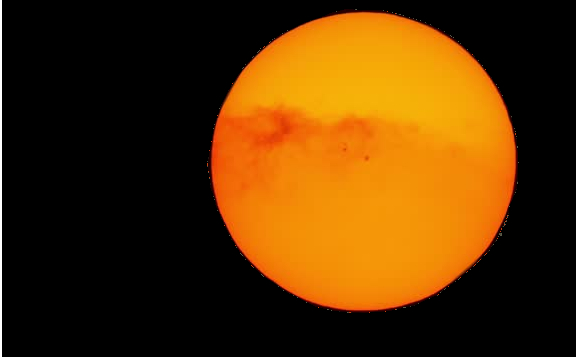
\includegraphics[width=0.4\textwidth]{img/orange.jpg}
		\caption{Наглядное изображение оранжевого круга на черном фоне}}
\end{figure}

\begin{figure}[ht!]%
    \centering
	\subfloat[A]{{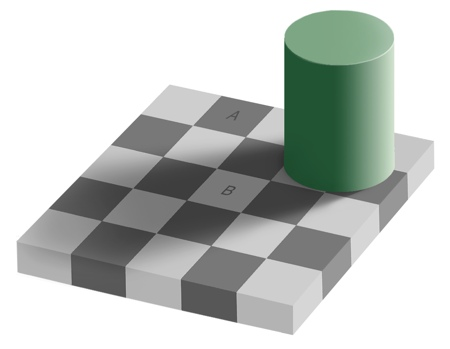
\includegraphics[width=6cm]{img/illusion_1.jpg} }}%
    \qquad
	\subfloat[B]{{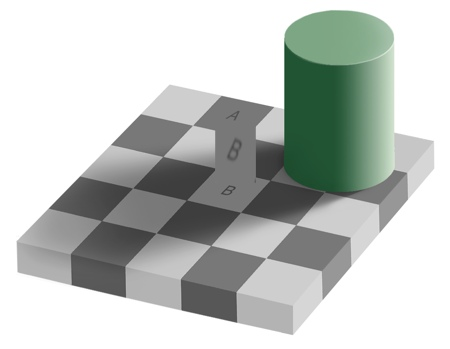
\includegraphics[width=6cm]{img/illusion_2.jpg} }}%
	\caption{Демонстрация психологических факторов человеческого восприятия(рисунок A-квадрат B кажется светлее квадрата A, но на самом деле они одного цвета(рисунок B))}%
\end{figure}

В работе будет рассматриваться первый случай, где не учитываются психологические аспекты человеческого восприятия. Следует выделить четкое понятие доминантного цвета.

\section{ Преобладающий цвет}
\textit{Доминантный(преобладающий) цвет} -- цвет, который представляет группу цветов пикселей, объедененных в единый кластер с помощью квантования. 

Данное понятие было введено в стандарте MPEG-7 в 2002 году, одним из визуальных дескрипторов которого является дескриптор доминантного цвета(DCD -- dominant color descriptor)

\section{ Цвет}
С физической точки зрения цвет представляет собой свет, который, отражаясь от объекта, попадает в глаз человека. Восприятие цвета человеком может зависить от психологического состояния индивида, от местоположения объекта, от строение глаза человека, от окружаещего света и т.д. То есть восприятяие цвета человеком достаточно субъективно. Свет в свою очередь можно описать как волну, длинна которой возбуждает разные рецепторы человеческого глаза. То есть, индивид будет понимать какого цвета объект перед ним в зависимости от того, в какой диапазон попадет длинна волны света, отраженного от этого объекта.

\subsection{ Цветовые модели и пространства}

Модель цвета -- абстрактная математическая модель представления цветов в виде кортежей чисел.

В какой-то момент необходимо было придумать модель цвета. Как и любое друго явление природы описать его так, чтобы цветовую информацию можно было удобно и эффективно использовть. Проблема описания цвета в форме математики была решена еще до появления компьютеров. Одним из первых таких описаний былa RGB(Red, Green, Blue) модель, идея которого заключалась в представлении всех цветов с помощью трех базовых понятий - красного, зеленого и синего. 

Цветовое пространство -- модель представления цвета, основанная на использовании цветовых координат. Цветовое пространство ориентировано на то, чтобы каждый оттенок модели был представлен в виде отдельной точки, имеющей свои собственные координаты. Например, каждая точка цветового пространства RGB имеет три координаты, которые характеризуют ее положение в пространстве, где каждая соответствует своей компоненте: красному, зеленому или синему.

RGB не является одним единственным пространством. Список основных цветовых пространств:
\begin{enumerate}
	\item RGB, sRGB, Adobe RGB
	\item CIEXYZ, CIELAB
	\item CMY(K)
	\item HSL, HSV
\end{enumerate}

\subsubsection{ RGB}
$RGB$ -- пространство характеризуется свойством аддитивности: стоится на составление цвета из трех базовых -- красного(Red), синего(Blue) и зеленого(Green).  Данное пространство часто называют цветовым кубом, потому что каждый базовый параметр цвета, представленного в этой модели, может восприниматься как координата трехмерного прямоугольного пространства.

\begin{figure}[ht!]%
    \centering
	\subfloat{{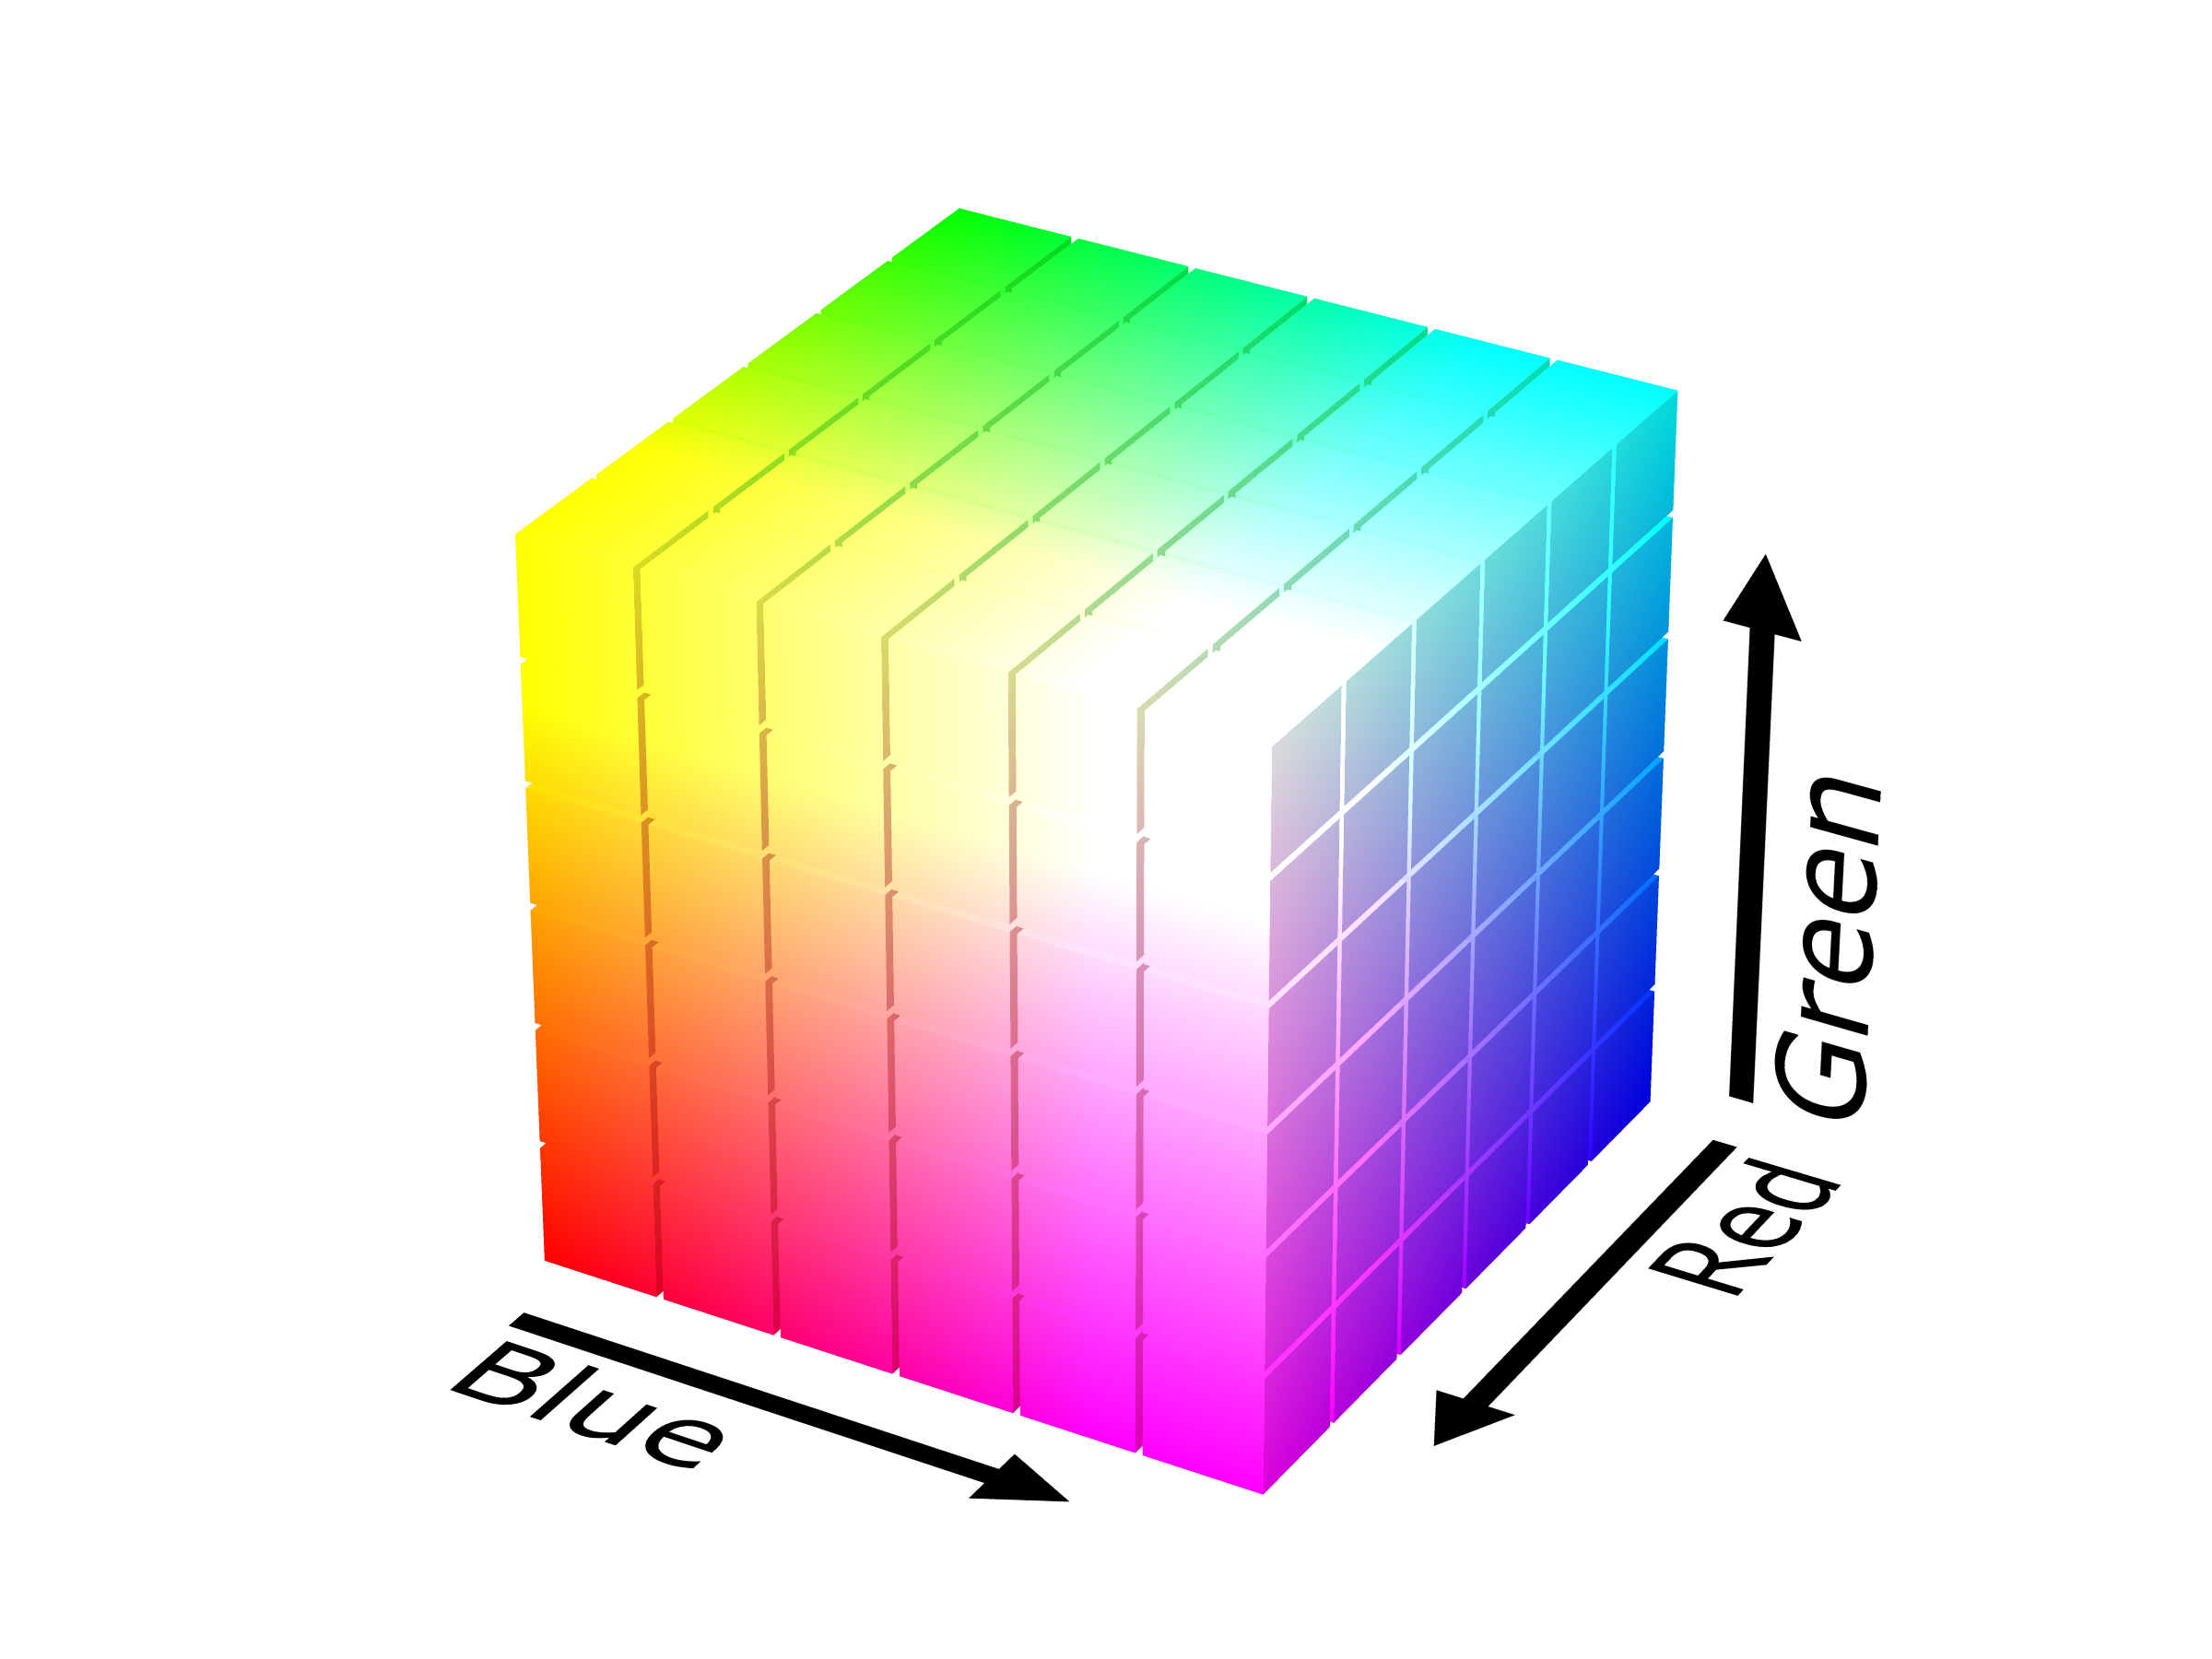
\includegraphics[width=6cm]{img/colorCubev2.png} }}%
    \qquad
	\subfloat{{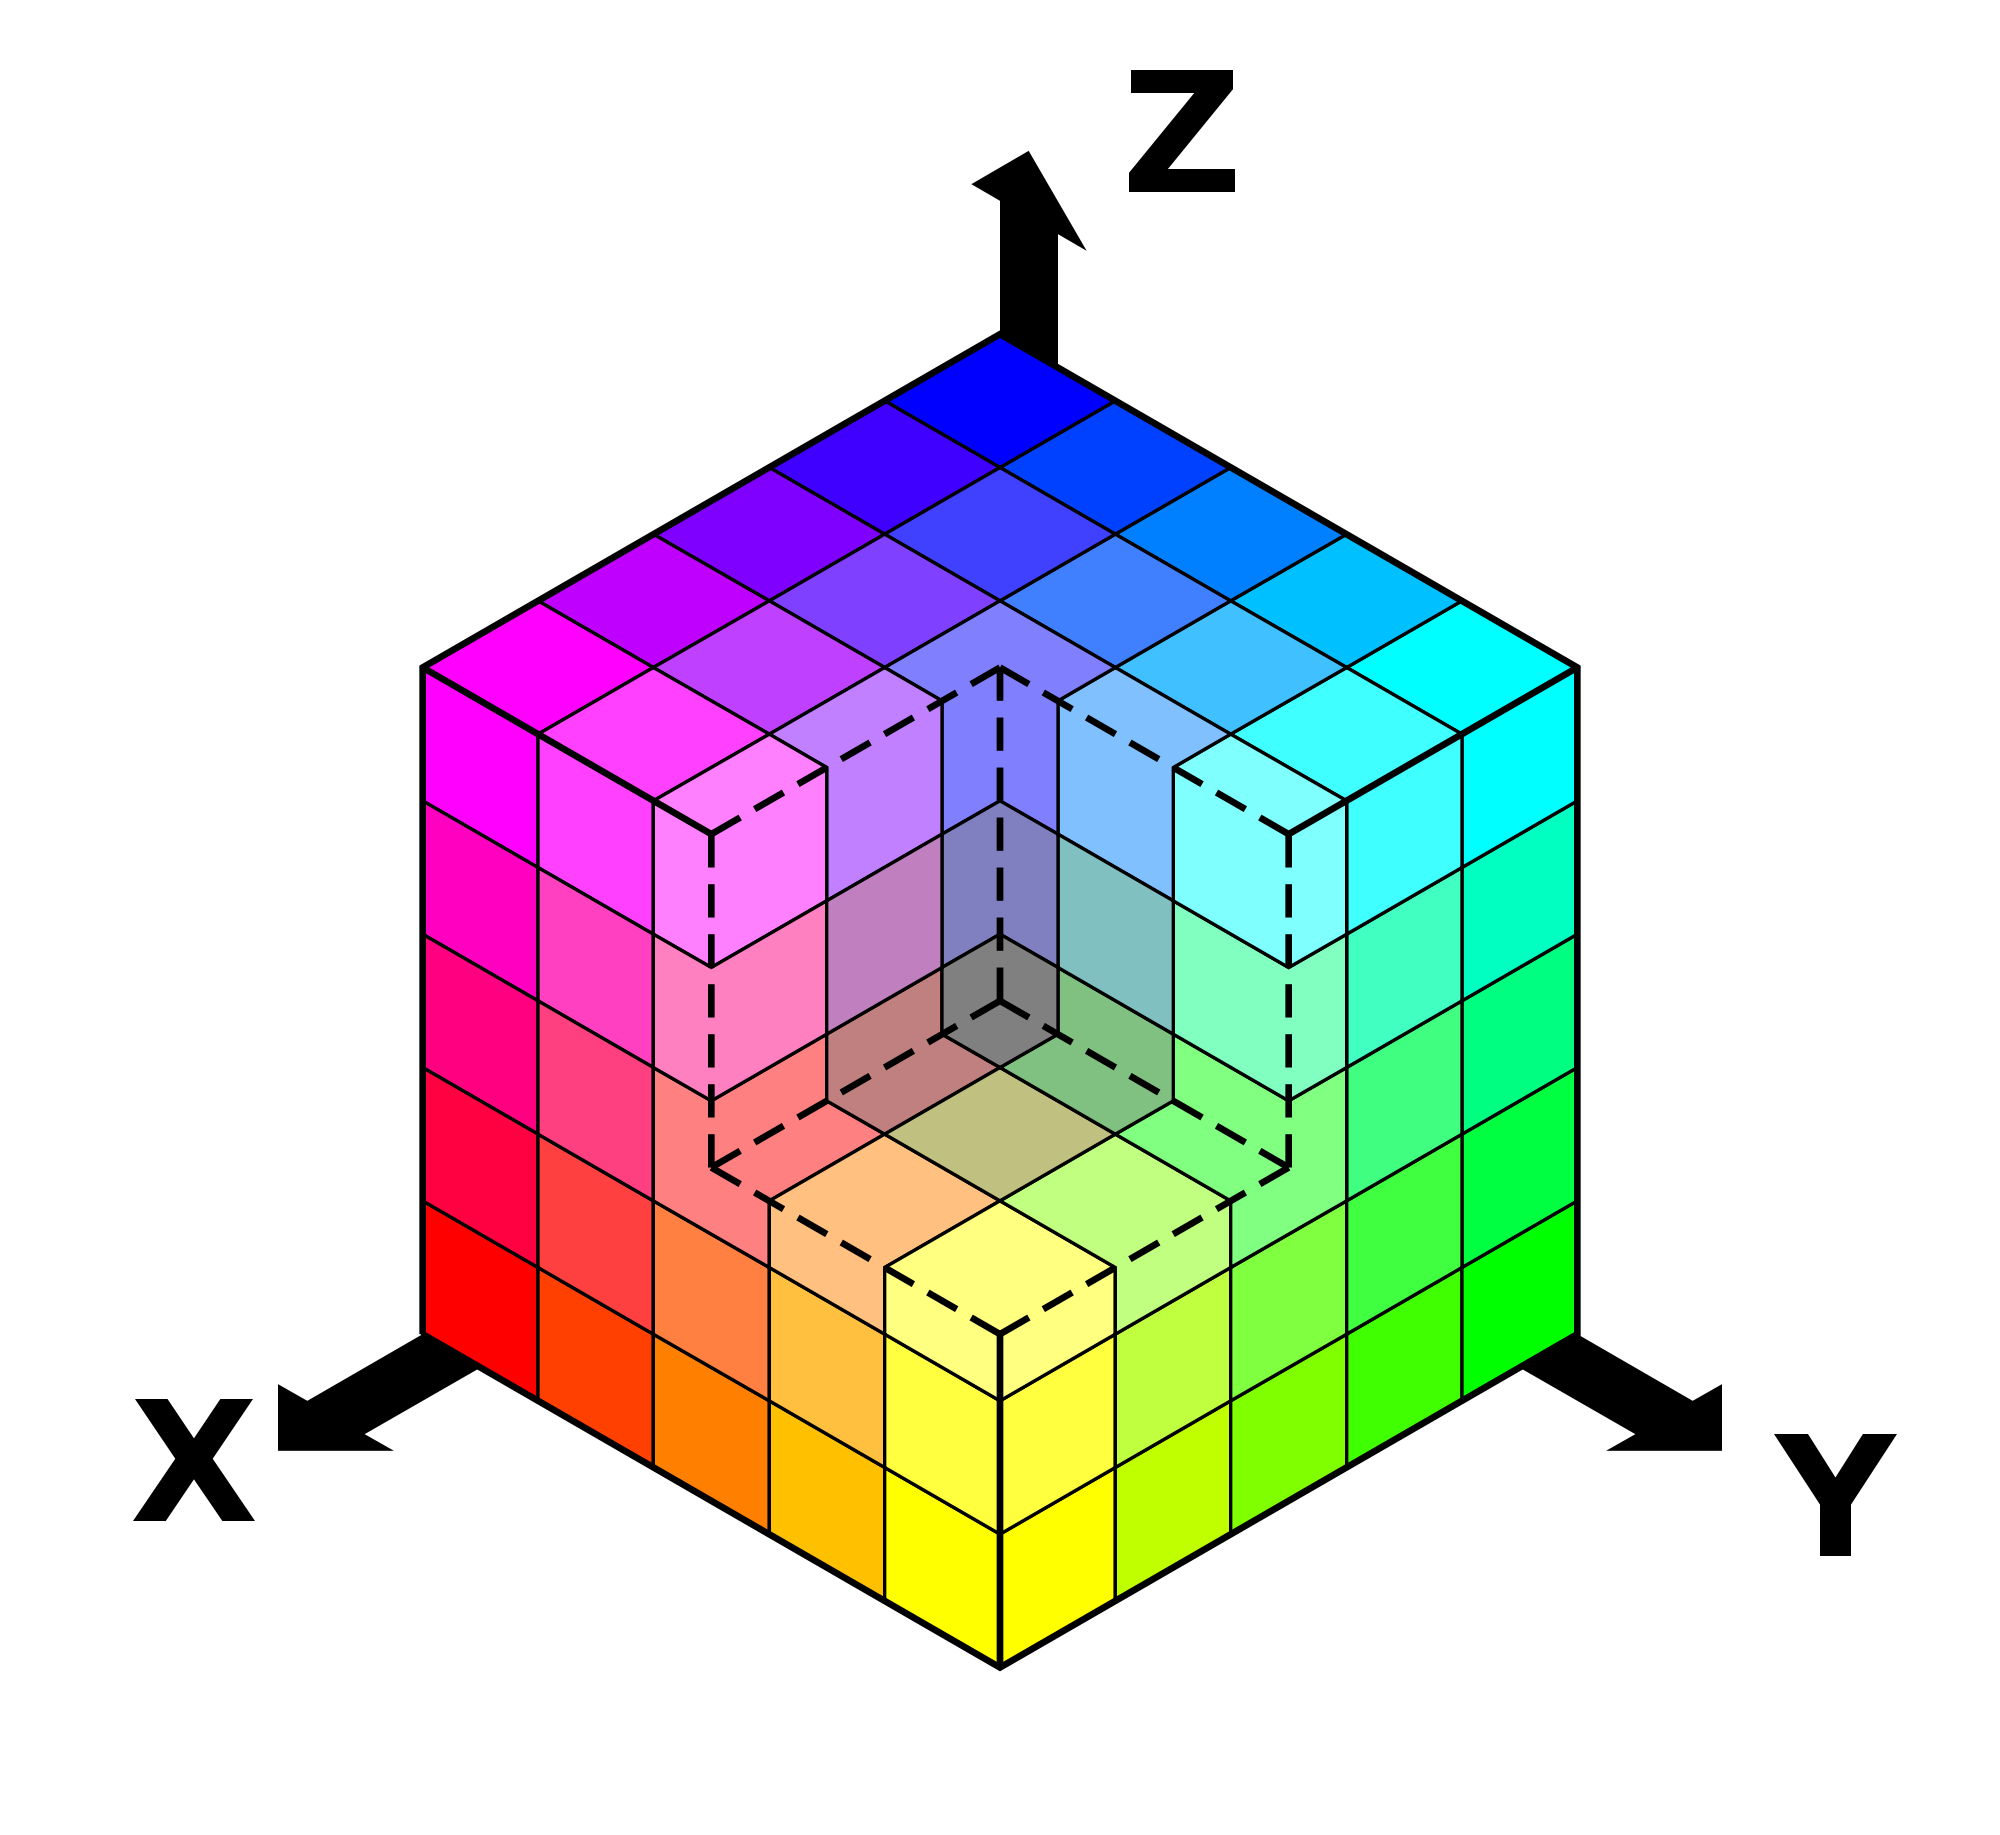
\includegraphics[width=6cm]{img/colorCubeSlice.png} }}%
	\caption{Представление цветового куба}%
\end{figure}

RGB пространство способно представить \(2^{24}\) = 16 777 216/\(2^8 * 2^8 * 2^8\) цветов(это может зависеть от качества графического оборудования). Числовые диапазоны значений(red, green, blue) могут быть представлены в разных видах: в процентах(от 0\% до 100\%), в виде действительных значений от 0 до 1(обычно используется при работе с цветовым кубом, при аналитических анализах), в виде целых чисел от 0 до 255(в компьютере информация представляется в виде битов и байтов)

Цветовая модель RGB была построена на основе закона Грассмана, который утверждает, что человек воспринимает свет линейно:

$\lambda$ -- длина волны. 

$I_1(\lambda)$ и $I_2(\lambda)$ -- спектральные функции, задающие источники света.

$I_h$ -- спектральная функция, задающая световой поток, который воспримет человек.

\begin{equation}
	I_h(\lambda) = I_1(\lambda) + I_2(\lambda)
\end{equation}

Спектральная функция $I(\lambda)$ -- функция, которая в общем виде описывает световой поток.

\subsection{ Проблема нахождения различий между цветами}
Большинство людей могут отличать цвета и их оттенки чисто визуально, опираясь на собственные цветовые ощущения. Листья деревьев, кирпичи дома -- все это содержит в себе оттенки одного цвета, который человек в состояние различить интуитивно.

Но компьютер не может опираться ни на какие ощущения, поэтому встает проблема нахождения различий между цветами. Как компьютер может определить, что цвета похожи или соверешнно разные?

Работая в цветовом пространстве, можно использовать Евклидово расстояние, но оно будет работать не так эффективно, как можте показаться. В большинстве случаев оно будет находить расстояние корректно(здесь уже все зависит от цветового пространства), но в некоторых цветовых пространствах могут возникнуть случаи, когда Евклидово расстояние в цветовом прострнастве между цветами будет одинаковым, но цвета, которые сравниваются, будут совершенно разными. Например, в RGB, в CMYK могут возникнуть такие ситуации.

\begin{figure}[ht!]
	\centering{
		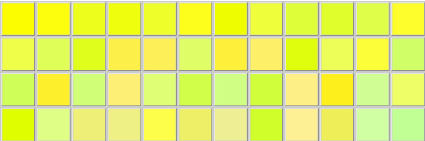
\includegraphics[width=0.4\textwidth]{img/EuclidianDifferenceRgb.png}
		\caption{Евклидовое расстояние, премененное к RGB}}
\end{figure}

\subsection{ Квантование цвета}
Квантование -- разбиение диапазона значений некоторой величины на конечное число уровней и округление этих значений до ближайших к ним уровней.

Квантование цвета в изображении важнейшая задача в поиске преобладающих цветов. Она позваляет уменьшить количество цветов отображаемой картинки. Это активно используется при сжатии, позволяя уменьшить цветовую палитру, при добавлении эффектов на изображение. Следующие алгоримы позволяют решить данную задачу:
\begin{enumerate}
	\item Линейно-блочный алгоритм, основанный на слиянии блоков(LBA -- Linear Block Algorithm).
	\item Алгоритм квантования цветов медианным сечением.
	\item Алгоритмы кластеризации(Например алгоритм k-средних).
\end{enumerate}

\subsubsection{ Алгоритм квантования цветов медианным сечением:}
Данный метод заключается в разбиении цветового пространства на параллелепипеды со сторонами, параллельными осям цветового пространства RGB.

Первый шаг заключается в нахождении минимального параллелепипеда, который содержит все цвета, представленые в изображении.

На втором шаге происходит определение самой длинной стороны параллелепипеда и сортировка всех значений вдоль выбранного направления. Далее параллелепипед разделяется по медиане множества значений выбранного направления на две части. Отсюда, получится два параллелепипеда, которые содержат примерно одинаковое количество значений. 

Предыдущая процедура повторяется до тех пор, пока не будет получено N параллелепипедов, где N - количество цветов новой палитры. После этого требуется заполнить палитру цветов, которая будет описывать изображение. Для каждого параллелепипеда нужно рассчитать цвет, который будет представлять его(либо центральная точка параллелепипеда, либо среднее арифметическое значение точек, попавших в него)

На самом изображении остается проанализировать пиксель(найти параллелепипед, в который попадает данная точка) и заменить цвет пикселя на цвет, который представляет весь параллелепипед.

\subsubsection{Алгоритм кластеризации k-средних:}
Метод кластеризации основан на центроидах -- точках, которые представляют собой центр кластера.

Первый шаг алгоритма заключается в инициализации центроидов, количество которых равно N(размер требуемой палитры). Инициализация центроидов очень важный момент, который сильно влияет на работу всего алгоритма. Можно взять случайные центроиды, но это возможно приведет к погрешности.

Далее выделяется два основных шага данного алгоритма: нахождение кластеров, которые определяются путем кратчайшего расстояние от точки до центроида, и рассчитывание центра масс получившихся кластеров, смещение центроидов на полученные центры масс. Эти два шага повторяются до тех пор, пока центроиды не стабилизируются и больше не будут смещаться.

\begin{figure}[ht!]
	\centering{
		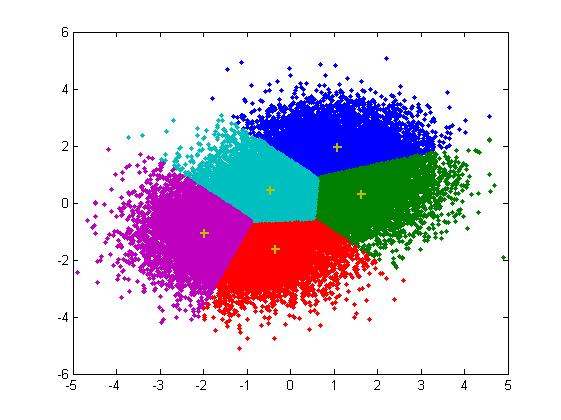
\includegraphics[width=0.4\textwidth]{img/k-means.jpg}
		\caption{Результат работы k-means с представленными центроидами}}
\end{figure}

\section{ Цветовые гистограммы}
Гистограмма -- график статического распределения цифрового изображения с различной яркостью, в котором по горизонтальной оси представлена яркость, а по вертикали -- относительное число пикселей с конкретным значением яркости. С помощью гистограммы определяется насыщенность изображения(либо сумарная, либо разделенная по цветовым каналам).

\begin{figure}[ht!]
	\centering{
		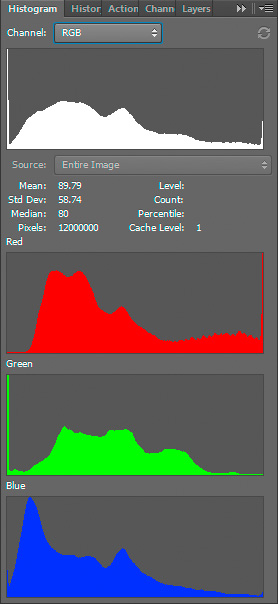
\includegraphics[width=0.4\textwidth]{img/histograms.jpg}
		\caption{Гистограммы, характеризующие изображение в программе Photoshop CS6}}
\end{figure}

\section{ MPEG-7}
MPEG-7 -- стандарт ISO/IEC, разработанный группой MPEG(Moving Picture Experts Group). Аббревиатура расшифровывается как Multimedia Content Description Interface(Мультимедиа-интерфейс для описания содержимого). Имеет цель стандартизировать и описать мультимедийное пространство.

Стандарт состоит из семи частей:
\begin{enumerate}
	\item Системы MPEG-7.
	\item Язык описания определений MPEG-7.
	\item Audio -- дескрипторы и схемы описания аудио материала.
	\item Visual -- дескрипторы и схемы описания визуального материала.
	\item Multimedia Descriptor Schemes -- дескрипторы и схемы описания общих характеристик описания мультимедиа.
	\item Reference Software -- програмные реализации соответствующих частей стандарта.
	\item Conformance -- базовые принципы и процедуры тестирования рабочих характеристик практических реализаций стандарта.
\end{enumerate}

\section{ Алгоритмы выделения преобладающего цвета}
\subsection{ Histogram algorithms}
\subsection{ GLA(generalized Lloyd Algorithm)}
\subsection{ Clustering algorithms}

\section{ Выбор подходящего алгоритма для решения задачи}
